\section{Introduction}
\label{sec:intro}

With the advance of device scaling technologies~\cite{3D-Nand,four-plane1}, the
capacity of flash-based SSDs has increased rapidly. The largest SSD was 1TB in
2013~\cite{1TB}, but as of 2022, a 32TB SSD is available in consumer
markets~\cite{32TB1,32TB2,32TB3}, and the biggest SSD reaches 100TB in
size~\cite{100TB}. This historical trend tells us that SSD capacity doubles
every year, so it is not surprising that a half-petabyte SSD would appear in
the near future. To enjoy such innovation in device capacity, however,
existing index structures for SSDs must be properly refactored.  

Because of the out-of-place update nature of NAND flash, existing
systems take a log-structured approach that appends incoming data to free
space~\cite{FTL-basic,flash-based-ssd}.  To locate data appended to the flash, the systems 
adopt a software layer, called flash translation layer (FTL), to maintain index structures that map 4KB logical blocks from the host to 4KB physical sectors in the flash.
The index structures are organized as a
logical-to-physical (L2P) table, which is kept in DRAM for fast lookups.
% \koo{The index structures are organized as a
% logical-to-physical (L2P) table, which is kept in DRAM for fast lookups.
% FTL 언급을 위해 위 문장을 다음 문장으로 변경 고려.
% Typically, a system software called flash translation layer (FTL),
% which is implemented in an SSD or kernel, organizes the index structure
% as a logical-to-physical (L2P) table, keeping it in DRAM for fast lookups.}
However, as SSD capacity gets larger, it becomes difficult to load an entire L2P table 
in DRAM. Considering that an L2P table size is roughly estimated as
0.1\% of SSD capacity~\cite{pink, dftl}, a high-density SSD (\eg~32TB) needs several
tens of GBs of DRAM (\eg~32GB).

Various index structures like hybrid~\cite{ superblockFTL, last, fast} and tree-based
indexing~\cite{uftl,utree} have been proposed to mitigate memory burden, but
they are not widely adopted because of high write amplification and wandering
tree problems~\cite{wandering-f2fs,wandering-b+}.  Instead, demand-based indexing is popularly
used.  It stores the entire table in the flash; instead, by caching only
popular entries with locality in DRAM, it provides reasonable performance with
small DRAM.  Some variants of demand-based indexing further improve memory
efficiency by delta-encoding table entries of logical blocks that are stored
over physically consecutive sectors.  The demand-based indexing, however, has
an intrinsic drawback; its read latency varies greatly depending on I/O
locality and system's condition.  If a workload has weak locality, it suffers
from degraded read latency by many cache misses.  Delta-encoding does not work
efficiently under fragmented storage space where logical blocks are scattered
across a wide range of physical sectors.

\begin{figure}[t]
    \centering
    \begin{subfigure}[b]{0.218\textwidth}
        \centering
        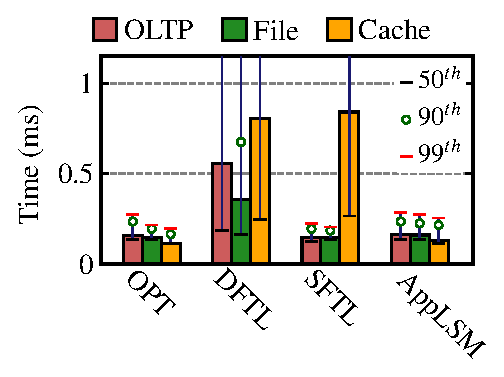
\includegraphics[width=\textwidth]{exp/no-tp-intro-a.eps}
        \vspace{-13.5pt}
   	    \caption{Impact of I/O locality}
        \label{fig:long-avg}
    \end{subfigure}
    \begin{subfigure}[b]{0.252\textwidth}
        \centering
        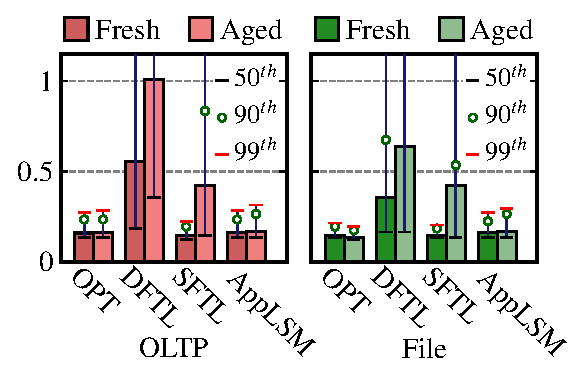
\includegraphics[width=\textwidth]{exp/new-aged-intro.eps}
        \caption{Impact of storage fragmentation}
        \label{fig:aged-oltp}
    \end{subfigure}
    \vspace{-15pt}
	%\caption{\koo{I/O latency of FTLs under OLTP, file, and cache systems}}
        \caption{Read latency of FTLs on various workloads}
	\label{fig:moti}
\end{figure}

To demonstrate the inconsistent latency of the demand-based indexing, we
evaluate two representative techniques, DFTL~\cite{dftl} and SFTL~\cite{sftl},
under three workloads: \texttt{OLTP}, \texttt{File}, and \texttt{Cache}.  We compare them with an
optimal FTL (OPT) that keeps an entire L2P table in DRAM, thereby offering
optimal performance without any extra I/Os.  DFTL has a limited size of DRAM to
cache only about 30\% of the total table entries.  SFTL uses the same DRAM but caches
more by delta-encoding entries.  All experiments are conducted using a PCIe SSD
prototype that offers the capacity of 512GB, 110$\mu$s read and 350$\mu$s write
latencies (see \SEC{sec:exp:setup} for detail).

\FIG{fig:moti}(a) shows the average read latency of different indexing techniques, along with their latency
at 50$^{th}$, 90$^{th}$, and 99$^{th}$ percentiles.  OPT presents consistent
I/O latency across all the workloads. Conversely, DFTL and SFTL experience a wide range of I/O latency depending on the workloads.
DFTL shows the worst performance
as it suffers from frequent cache misses, which results in many I/Os to load
missing entries.  The system condition also significantly affects I/O latency.
\texttt{OLTP} and \texttt{File} have moderate spatial locality, so SFTL can
efficiently coalesce consecutive table entries.  However, if the same workload
runs on the aged file system severely fragmented with many free-space holes,
SFTL shows degraded performance (see \FIG{fig:moti}(b)).  Under the fragmented
file system, data are likely to be scattered across free-space holes, which
makes delta-encoding inefficient.

This inconsistent I/O latency is considered harmful, particularly in
enterprise environments where consistent service quality is
paramount~\cite{cloud, silk, udepot}.  SSD vendors are thus reluctant to adopt the
demand-based indexing for enterprise-grade products. Instead, they walk around
the problem just by keeping a huge L2P table in DRAM. This simple remedy,
however, will not work anymore, considering that SSD capacity keeps increasing,
reaching several hundreds of TBs.

This paper proposes approximate LSM-tree indexing, \textit{\ours{}}, 
for ultra-scale SSDs to provide consistent and low I/O latency
regardless of I/O locality and system's conditions.
\ours{} differs from existing index structures in three aspects. 
\begin{itemize}[leftmargin=*]
\item{\textbf{Adoption of an LSM-tree for Indexing.}}
An LSM-tree is a hierarchical structure that consists of multiple 
levels, each of which stores data
in a \emph{sorted} and \emph{append-only} way.
%Such inherent characteristics of an LSM-tree require 
%a much smaller memory for L2P indexing 
%as compared to a flat structure and 
Such inherent characteristics of an LSM-tree give
us an opportunity to reduce required memory for L2P indexing
and do not suffer from the wandering tree problem 
imposed on typical tree structures~\cite{wandering-f2fs}.
To the best of our knowledge, 
this is the first work that uses an LSM-tree for L2P indexing.

\item{\textbf{Use of Approximate Indices.}}
Instead of maintaining a huge number of exact indices 
that map all logical blocks to corresponding physical sectors 
by one-to-one, \ours{} uses a few approximate indices 
to infer corresponding physical sectors of target logical blocks.
Combined with the sorted property of an LSM-tree, 
approximate indices can be built in a highly memory-efficient manner,
exhibiting \koo{4.1}--8.4$\times$ lower memory footprints 
than typical exact indices.

\item{\textbf{No Caching.}}
By leveraging the memory-efficient nature of approximate indices,
\ours{} can keep entire indices in small DRAM.
The performance of \ours{} is thus never affected by external factors,
such as I/O locality and system's condition, 
resulting in consistent I/O latency.
\end{itemize}

\begin{comment}
This paper proposes approximate LSM-tree indexing, \textit{\ours{}}, 
for ultra-scale SSDs to provide consistent and low I/O latency
regardless of I/O locality and system's conditions.
%\hs{To the best of our knowledge, this is the first work that employs an LSM-tree along with approximation for translating logical blocks to physical sectors for SSDs.}
\ours{} differs from existing index structures in three aspects. 
(\textit{i}) The first is
the adoption of an LSM-tree~\cite{lsm-tree} for indexing.
An LSM-tree is a hierarchical structure that consists of multiple 
levels, each of which stores data
in a \emph{sorted} and \emph{append-only} way, respectively.
%Such inherent characteristics of an LSM-tree require 
%a much smaller memory for L2P indexing 
%as compared to a flat structure and 
Such inherent characteristics of an LSM-tree give
us an opportunity to reduce required memory for L2P indexing
and do not suffer from the wandering tree problem 
imposed on typical tree structures~\cite{wandering-f2fs}.
% The append-only nature of an LSM-tree 
% is not only suitable for the physical property of the flash,
% but also does not cause the wandering tree problem that typical tree structures impose~\cite{wandering-f2fs}.
(\textit{ii}) The second is the use of approximate indices.
Instead of maintaining a huge number of exact indices 
that map all logical blocks to corresponding physical sectors 
by one-to-one, \ours{} uses a few approximate indices 
to infer the corresponding physical sectors of target logical blocks.
Combined with the sorted nature of an LSM-tree, 
approximate indices can be built in a highly memory-efficient manner,
which exhibits 4.7--8.4$\times$ lower memory footprints 
than typical exact indices.
(\textit{iii}) The third is no caching. 
By leveraging the memory-efficient nature of approximate indices,
\ours{} can keep entire indices in small DRAM.
The performance of \ours{} is thus never affected by external factors,
such as I/O locality and system's condition, 
resulting in consistent I/O latency.
%\hs{Tightly integrating all the above features is not only novel but also crucial to achieve the goal. 
%This is because a lack of either an LSM-tree or approximation typically inflates memory footprints for indexing, making I/O latency hardly consistent.}
\end{comment}

To efficiently combine approximate indices with an LSM-tree, we
must address the following three issues.  
The first is the design of memory-efficient yet accurate approximate algorithms.
Approximate indices inevitably result in prediction errors, which may cause extra I/Os.
To minimize the negative impact of errors,
we design fingerprint (FP)- and piecewise linear regression (PLR)-based
approximation algorithms~\cite{plr1,plr2, plr3} and
optimize them using various techniques 
to provide a bounded error rate with minimal DRAM usage.
% they provide 
% a low error rate with minimal DRAM usage.  

The second is the CPU overhead of utilizing
approximate indices.
We optimize the read
path of \ours{} so that index lookups are served with a few bit-wise or
arithmetic operations.  
We also construct approximate indices by using cheap hash functions and hide the construction overhead by interleaving with I/Os.
% Approximate indices are constructed quickly by
% invoking cheap hash functions and interleaving with I/Os.  

The third is high I/O amplification
of an LSM-tree. This is caused by a hierarchical structure of an LSM-tree
that requires to look up multiple levels in the tree before reading target data~\cite{lsm-tree}. 
We address this problem by introducing a tiny DRAM-resident table,
eliminating a tree traversal. To maintain the tree
sorted, an LSM-tree also requires to perform the compaction process
that involves extra writes~\cite{lsm-tree}.
% to move previously written data elsewhere~\cite{lsm-tree}. 
With a careful design of a tree hierarchy along with a different choice of approximation algorithms at each level, 
% By organizing a tree hierarchy and optimizing the compaction process,
\ours{} is able to efficiently reduce the compaction overhead, providing 
write throughput comparable to state-of-the-art techniques.  

We implement \ours{} in an FPGA-based OCSSD prototype and 
carry out experiments using various workloads, Filebench~\cite{filebench}, 
YCSB~\cite{ycsb}, TPC-C~\cite{TPC-C}, and CacheLib~\cite{cachelib},
comparing
\ours{} to the state-of-the-art indexing techniques, including the optimal
FTL~\cite{flash-based-ssd}, DFTL~\cite{dftl}, SFTL~\cite{sftl}, and TPFTL~\cite{tpftl}.
Our experimental results show that, given a target error rate of 0.1, \ours{} exhibits read latency
close to that of the best-performing optimal FTL.
This is achieved 
by using much less DRAM (29.1\%) than the optimal FTL requires.  
\ours{} outperforms the demand-based indexing approaches, 
achieving up to 46.1\% and 47.3\%
shorter average and $99^{th}$ read latency, respectively.  The throughput of \ours{}
is slightly higher than or similar to that of the demand-based indexing approaches under write-heavy workloads. 
To confirm the feasibility of
\ours{}, we also port the \ours{} prototype to a Cortex
A53-based SSD controller and evaluate its time complexity.


%\fixme{(기여를 요약하는게 좋을 듯;
%1) 새로운 LSM-tree 기반의 approximate indexing structure 제안)
%2) 메모리 사용량을 극단적으로 줄이는 반면 읽기 성능 보장,
%3) Tree 구조 조절을 통한 WAF 악화 방지 (Log-buffer의 단점으로 high WAF 언급),
%4) 실제 구현 및 평가}

%The rest of this paper is organized as follows: In \SEC{sec:back}, we review
%background related to this study.  After explaining the overall design of
%\ours{} in \SEC{sec:overall}, we present the details of approximate indexing algorithms
%in \SEC{sec:design}.
%We then explain implementation issues in \SEC{sec:impl}. After showing the results in
%\SEC{sec:exp}, we conclude in \SEC{sec:con}.



% With the advance of device scaling technologies~\cite{3D-Nand,four-plane1}, the
% capacity of flash-based SSDs has increased rapidly. The largest SSD was 1TB in
% 2013~\cite{1TB}, but as of 2022, a 32TB SSD is available in consumer
% markets~\cite{32TB1,32TB2,32TB3}, and the biggest SSD reaches 100TB in
% size~\cite{100TB}. This historical trend tells us that SSD capacity doubles
% every year, so it is not surprising that a half-petabyte SSD would appear in
% the near future. To enjoy such innovation in device capacity, however,
% existing index structures for SSDs must be properly refactored.  

% Because of the out-of-place update property of NAND flash, existing
% systems take a log-structured approach that appends incoming data to free
% space~\cite{FTL-basic, flash-based-ssd}.  To locate data appended to the flash, the systems 
% adopt a software layer, called flash translation layer (FTL), to maintain index structures that map 4-KB logical blocks from the host to 4-KB physical sectors in the flash.
% The index structures are organized as a
% logical-to-physical (L2P) table, which is kept in DRAM for fast lookups.
% % \koo{The index structures are organized as a
% % logical-to-physical (L2P) table, which is kept in DRAM for fast lookups.
% % FTL 언급을 위해 위 문장을 다음 문장으로 변경 고려.
% % Typically, a system software called flash translation layer (FTL),
% % which is implemented in an SSD or kernel, organizes the index structure
% % as a logical-to-physical (L2P) table, keeping it in DRAM for fast lookups.}
% However, as SSD capacity gets larger, it becomes difficult to load an entire L2P table 
% in DRAM. Considering that an L2P table size is roughly estimated as
% 0.1\% of SSD capacity~\cite{pink, dftl}, a high-density SSD (\eg~32TB) needs several
% tens of GBs of DRAM (\eg~32GB).

% Various index structures like hybrid~\cite{ superblockFTL, last, fast} and tree-based
% indexing~\cite{uftl,utree} have been proposed to mitigate memory burden, but
% they are not widely adopted because of high write amplification and wandering
% tree problems~\cite{wandering-f2fs,wandering-b+}.  Instead, demand-based indexing is popularly
% used.  It stores the entire table in the flash; instead, by caching only
% popular entries with locality in DRAM, it provides reasonable performance with
% small DRAM.  Some variants of the demand-based indexing further improve memory
% efficiency by delta-encoding table entries of logical blocks that are stored
% over physically consecutive sectors.  The demand-based indexing, however, has
% an intrinsic drawback; its read latency varies greatly depending on I/O
% locality and system's condition.  If a workload has weak locality, it suffers
% from degraded read latency by many cache misses.  Delta-encoding does not work
% efficiently under fragmented storage space where logical blocks are scattered
% across a wide range of physical sectors.

% \begin{figure}[t]
%     \centering
%     \begin{subfigure}[b]{0.218\textwidth}
%         \centering
%         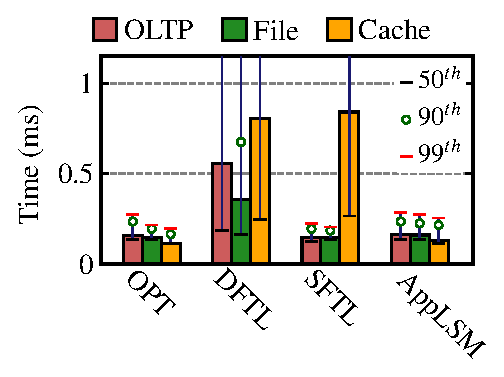
\includegraphics[width=\textwidth]{exp/no-tp-intro-a.eps}
%         \vspace{-13.5pt}
%    	    \caption{Impact of I/O locality}
%         \label{fig:long-avg}
%     \end{subfigure}
%     \begin{subfigure}[b]{0.252\textwidth}
%         \centering
%         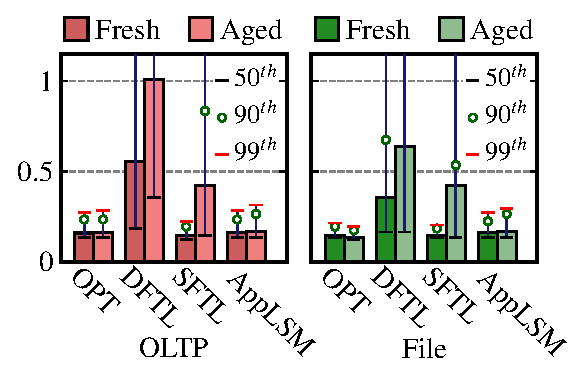
\includegraphics[width=\textwidth]{exp/new-aged-intro.eps}
%         \caption{Impact of storage fragmentation}
%         \label{fig:aged-oltp}
%     \end{subfigure}
%     \vspace{-15pt}
% 	%\caption{\koo{I/O latency of FTLs under OLTP, file, and cache systems}}
%         \caption{\koo{Read latency of FTLs on various systems}}
% 	\label{fig:moti}
% \end{figure}

% To demonstrate the inconsistent latency of the demand-based indexing, we
% evaluate two representative techniques, DFTL~\cite{dftl} and SFTL~\cite{sftl},
% under three workloads: OLTP, file, and cache systems.  We compare them with an
% optimal FTL (OPT) that keeps an entire L2P table in DRAM, thereby offering
% optimal performance without any extra I/Os.  DFTL has a limited size of DRAM to
% cache only \JS{about} 30\% of the total table entries.  SFTL uses the same DRAM but caches
% more by delta-encoding entries.  All experiments are conducted using a PCIe SSD
% prototype that offers the capacity of 512GB, 110$\mu$s read and 350$\mu$s write
% latencies (see \SEC{sec:exp:setup} for detail).

% \FIG{fig:moti} shows the average latency of the FTLs, along with their latency
% at 50$^{th}$, 90$^{th}$, and 99$^{th}$ percentiles.  OPT presents consistent
% I/O latency across all the workloads. Conversely, DFTL and SFTL show diverse
% I/O performance depending on the workloads.  DFTL shows the worst performance
% as it suffers from frequent cache misses, which results in many I/Os to load
% missing entries.  System's condition also significantly affects I/O latency.
% \texttt{OLTP} and \texttt{File} have moderate spatial locality, so SFTL can
% efficiently coalesce consecutive table entries.  However, if the same workload
% runs on the aged file system severely fragmented with many free-space holes,
% SFTL shows degraded performance (see \FIG{fig:moti}(b)).  Under the fragmented
% file system, data are likely to be scattered across free-space holes, which
% makes delta-encoding inefficient.

% Such inconsistent I/O latency of SSDs is considered harmful particularly in
% enterprise environments where consistent service quality is
% paramount~\cite{cloud, silk, udepot}.  SSD vendors are thus reluctant to adopt the
% demand-based indexing for enterprise-grade products. Instead, they walk around
% the problem just by keeping a huge L2P table in DRAM. This simple remedy,
% however, will not work anymore, considering that SSD capacity keeps increasing,
% reaching several hundreds of TBs.

% This paper proposes approximate LSM-tree indexing, \textit{\ours{}}, 
% for ultra-scale SSDs.  \ours{} differs from
% existing index structures in three aspects.  \JS{\textit{(i)} The first is
% the adoption of an LSM-tree~\cite{lsm-tree} for indexing}.
% The append-only nature of an LSM-tree 
% is not only suitable for the physical property of the flash,
% but does not cause the wandering tree problem that typical tree structures impose~\cite{wandering-f2fs}.
% \JS{\textit{(ii)} The second is the use of approximate indices}.
% Instead of large indices pointing to exact locations of data,
% \ours{} uses only approximate indices 
% to infer locations of data in the read path.
% Combined with the sorted nature of an LSM-tree, 
% approximate indices can be built in a highly memory-efficient manner,
% which exhibits 4.7--8.4$\times$ lower memory footprints than typical exact indices.
% \JS{\textit{(iii)} The third is no caching}. By leveraging the space-efficient nature of approximate indices,
% \ours{} can keep entire indices in small DRAM.
% The performance of \ours{} is thus never affected by external factors,
% such I/O locality and system's condition, which result in cache misses.

% To efficiently combine approximate indices with an LSM-tree, we
% must address following three issues.  
% The first is the design of memory-efficient yet accurate approximate algorithms.
% Approximate indices inevitably result in prediction errors, which may cause extra I/Os.
% To minimize a negative impact of errors,
% we design fingerprint (FP)- and piecewise linear regression (PLR)-based
% approximation algorithms~\cite{plr1,plr2, plr3} and 
% optimize them using various techniques, so that
% they provide 
% a low error rate with minimal DRAM usage.  

% The second is CPU overhead of looking up and building
% approximate indices.
% We optimize the read
% path of \ours{} so that index lookups are served with a few bit-wise or
% arithmetic operations.  Approximate indices are constructed quickly by
% invoking cheap hash functions or are built in a manner
% that hides its overhead through interleaving with I/Os.  

% The third is high I/O amplification
% of an LSM-tree. This is caused by a leveled organization of an LSM tree
% that requires to \koo{look up} multiple levels in the tree before reading wanted data~\cite{lsm-tree}. 
% We address this problem by introducing a tiny DRAM-resident table, called a
% shortcut table. To make the tree
% sorted, an LSM-tree also has to perform compaction
% that involves extra writes to move previously written data elsewhere~\cite{lsm-tree}. 
% By organizing a tree hierarchy and optimizing a compaction process,
% \ours{} is able to bound compaction costs, offering 
% write throughput comparable to state-of-the art
% techniques.  

% We implement \ours{} in an FPGA-based OCSSD prototype and 
% carry out experiments using various workloads, Filebench~\cite{filebench}, 
% YCSB~\cite{ycsb}, TPC-C~\cite{TPC-C}, and CacheLib~\cite{cachelib},
% comparing
% \ours{} to the state-of-the-art translation\JS{indexing?} techniques, including the optimal
% FTL~\cite{ostep:ssd}, DFTL~\cite{dftl}, SFTL~\cite{sftl}, and TPFTL~\cite{tpftl}.
% Our results show that, given a target error rate of 0.1, \ours{} exhibits read latency
% close to that of the best-performing optimal FTL.
% This is achieved 
% by using much less DRAM (29.1\%) that the optimal FTL needs.  
% \ours{} outperforms the demand-based indexing, 
% achieving up to 46.1\% and 47.3\%
% shorter average and $99^{th}$ read latency.  The throughput of \ours{}
% is slightly higher than or similar to the demand-based indexing under write-heavy workloads. 
% To confirm the feasibility of
% \ours{}, we also port the \ours{} prototype to a Cortex
% A53-based SSD controller and evaluate its time complexity.